% !TEX encoding = UTF-8
% !TEX TS-program = pdflatex
% !TEX root = ./thesis.tex
% !TEX spellcheck = en

%************************************************



\section{Automated information gathering} 
%\color{green}    trovare strutture, anche per mezzo di algoritmi di data mining
\color{red}    
The World Wide Web is the largest and most widely known repository of hypertext. Hypertextual documents (also called web documents or web pages) contain information about every topic and every real-world entity, authored and edited by millions of people and written in hundreds of languages. Moreover, hyperlinks creating billions of connections among web pages make the Web the largest and the most connected information network, where information in form of facts, ideas, and opinions are splitted and propagated among pages.  

How to gather, extract and merge useful
and meaningful information from the Web, however, becomes challenging to web
users. 
%This challenging issue is referred by many researchers as Web information gathering [23,11]. Given an information needs, Web information gathering aims to acquire useful and meaningful information for users from the Web.
%The information gathering in this huge and distributed data source is not a trivial task.
 In fact, access to web information is directly opposite to what we know from databases and libraries, where all data items or documents are well organized (in types, topics, area, years, etc.) and structured (e.g. tables). 
 
Currently, there
are two predominant and complementary paradigms for users to locate information: \emph{i)} Keyword-based search and \emph{ii)} Navigation paradigm \cite{Olston:2003, Fang:2007, Kalbach:2007, Levene:2010}. In the keyword-based search paradigm, the user types a search query (usually a list of key terms) into a search engine and obtains a ranked list of pages in descending order of relevance and accuracy respect to the input query.  
Nowadays, most websites provide embedded search engine for quickly identifying pages containing specific information.
The main drawback of this paradigm is that users have to know what they are looking for. In fact, for expressing information needs to the search engine, users have to think of appropriate key terms. Therefore, this paradigm is useful when users are familiar with the search domain (e.g., when they know the best terms to express their information needs and discriminate as much as possible their search domain from other domains). In all the other cases, when for example users do not know what they are looking for until the available options are presented or when their information needs cannot be formulated in keywords, this paradigm results unusable for the information gathering purpose~\cite{Lee:2005, Olston:2003}.

In the navigation paradigm, users start with the homepage or a web page found through a search engine or linked from another website, and then use the navigation systems (e.g. sitemaps, navbar, menu, etc.) provided by the website to find the desired information. %Studies reveal that users not randomly explore web pages in a website, but proceed in a top-down fashion, from a more general page to a detailed page using links of navigation systems with higher frequency compared to the other links of web graph~\cite{Anderson:2001,Amadieu:2010, Wang:2011, Weninger:2012}. 
The main drawbacks of this paradigm are the consuming time for finding specific information and the risk of get lost in the hyperspace. %which is one of the central unresolved problems of web interaction.
Getting lost comes from a feeling of frustration of not finding the information we are looking for and from a feeling of disorientation within the web site we are surfing through. To decrease this problem, several data mining tools are developed to increase the website usability and user interaction.
Analogously to the diverse set of tools ranging from road signs, the compass and map, to global positioning systems (GPS), all of which we use to orient ourselves in physical spaces, these solutions allow web users to understand in the hyperspace where they are, where they can go and where they come from ~\cite{Nielsen:2006}.

Information gathering is a challenging task also for machines. In fact, differently from web users, machines cannot easily understand the information codified in web pages. % such as structured data and the rest of the web content. 
This is due by the fact that HTML code is used for data visualization rather than data representation. By this, we mean that humans can easily distinguish e.g. main and secondary menus, navbars, breadcumbs, product listing, advertisements, unstructured contents based on web page visual features and position. Machines in contrast cannot directly extract these semantics~\cite{Keller:2013}. To overcome this issue two main solutions are possible: \emph{i)} using data markup to encode machine-readable knowledge (e.g. semantic formalization for structured data specified by
Schema.org\footnote{Schema.org is an initiative of the major search engine operators for creating, maintaining, and promoting schemas for structured data on the Internet, on web pages, etc.. See \url{http://schema.org/}.}); \emph{ii)} novel data mining methods to extract structured information~\cite{Lanotte:2014}, to infer a structure or a schema for data codified in web pages~\cite{Zhai:2005}, and to facilitate data mash-up~\cite{Dong:2014, Bronzi:2013}. Then, information extracted by data mining tools can be used for helping web users in the information gathering process (e.g. clustering similar web pages and extracting the logical structure of websites such as sitemaps). 

To summarize, the challenge of data mining tools for helping web users is to automate the information gathering process. For this scope, existing solutions try to bring back the semantic and structure of the Web and its web pages in the way that users and machines can easily access and use the vast amount of information available. For this scope several research fields are involved, such as Web Mining \cite{Chevalier:2008}(which analyze web pages' contents, hyperlinks and user logs), Web Information extraction~\cite{Dalvi:2012} (which extract information in form of structured data), Sequential pattern mining \cite{Mooney:2013}(for extracting recurrent patterns), Network Analysis~\cite{Sun:2012} (which evaluates how information is propagated in the Web), etc. .



%Continuare di qui \color{blue} dATA MINING THE WEB Uncovering Patterns in Web Content, Structure, and Usage
\color{red}
\section{Mining the Web}
%Papers da vedere:
%\begin{itemize}
%\item Mining the Web, discovering knowledge hypertex data
%\item Web Data Mining Trends and Techniques
%\item Automated Information Extraction from Web
%Sources: a Survey (classificazione web pages)
%\item Web Data Mining, Bing Liu
%item \url{https://www.researchgate.net/publication/266275732_Discovering_Web_Page_Communities_for_Web-Based_Data_Management}
%\item \url{http://arxiv.org/pdf/cs/0011033.pdf} Web Mining Research: A Survey
%\item \url{http://citeseerx.ist.psu.edu/viewdoc/download?doi=10.1.1.517.3557&rep=rep1&type=pdf} analisi dei grafi
%\end{itemize}
\color{red}
%The World Wide Web is the largest and most widely known repository of hypertext. Hypertextual documents (also called web documents or web pages) contain information about every topic and every real-world entity, authored and edited by millions of people and written in hundreds of languages. Moreover, hyperlinks creating billions of connections among web pages make the Web the largest and the most connected information network, where information in form of facts, ideas, and opinions are splitted and propagated among pages.  

%However, the Web represents also the largest social network where authors and writers, responsible for building without censure new facts, ideas, and opinions or modify them, are able to influence a same number of readers, responsible to propagate this knowledge.\\

%The Web has many unique characteristics which make Web Mining, defined as the automatic discovery of interesting and valuable information from web sources, an interesting and challenging task~\cite{Liu:2006}. In the following the main characteristics of the Web are analyzed:

The Web has many unique characteristics which make the discovering of novel and valuable information an interesting and challenging task~\cite{Liu:2006}. These characteristics can be summarized as follows: 
\begin{itemize}
\item \textbf{Dimension}. The amount of data and information on the Web is huge and still growing. The Web is the first medium where the number of information producers, responsible for building without censure new facts, ideas, and opinions, is the same magnitude order of information consumers. Published datasets are so large and complex that traditional data processing applications are inadequate to deal with them. Challenges include analysis, capture, data curation, search, sharing, storage, transfer, visualization, querying, updating and information privacy. 
\item \textbf{Dynamicity}. Each second thousands of web pages are created, destroyed and modified. This make the Web a dynamic information network, where
 the structure and the content change frequently. Keeping up with these changes and monitoring them are important issues for many applications. 
\item \textbf{Heterogeneity}. Web pages are heterogeneous in terms of formats and writing styles. In the first case, the heterogeneity is due by the fact that web pages do not respect a standard format. In fact, they can be classified in three categories~\cite{Chang:2006}: i) unstructured pages; ii) structured pages; iii) semi-structured pages. \\
\textit{Unstructured pages}, also called free-text documents, are written in natural language. No structure can be found, and only information extraction (IE) techniques can be applied with a certain degree of confidence \cite{Sarawagi:2008}. \\
\textit{Structured pages} are normally obtained from structured data sources (e.g., databases) and data are published together with their schema. %information on their structure. 
In general, information extraction on structured pages is accomplished using techniques based on syntactic matching. \\
\textit{Semi-structured pages} are in an intermediate position between unstructured and structured pages. These documents possess anyway a kind of structure which is enclose in free-text. Extraction techniques are often based on the presence of regular patterns as HTML tags, CSS code, etc. ~\cite{Ferrara:2012}.\\
Heterogeneity of web pages is also due by the presence of different and informal writing styles \cite{Liu:2006, Kim:2012}. In fact, differently from a traditional textual collection, web pages are created by millions of people having different cultures, skills, languages, etc.. This means that web pages may present the same or similar information using completely different words and/or formats. This makes extraction and integration of information from multiple pages a challenging problem. 

\item \textbf{Connection}. The Web is generally represented as an information network, that is a graph, where nodes are web pages and edges are hyperlinks. Hyperlinks in the Web have several roles and functionality. In particular, hyperlinks between pages belonging to the same website (e.g., domain) codify the navigation systems of the website (e.g., menus, navbars, sitemaps, etc.). In other words, they serve as mechanisms to coherently organize the information within the website and assist users during the website's navigation. Differently from hyperlinks belonging to a single website, hyperlinks across different websites encode latent human judgments of authority to the target pages~\cite{Levene:2010}. In this case, a link represents a concrete indication of the following type of judgment: the creator of page $p$, by including a link to page $q$, has in some measure conferred authority (i.e., trust) on $q$. According with this idea it is possible identify in the information network \emph{authoritative pages}, which provide good information, and \emph{hub pages}, which provide links to good
authorities pages. %In this case, links to authority pages are based on the assumption that as humans we have trust in veracity of these kind of pages.
 
\item \textbf{Noise}. 
The richness of information has also made the Web progressively more difficult to leverage the value of information. Differently from other media, information publication in the Web does not require editorship and approval from some authority. 
This unregulated atmosphere contributes not only to the big volume and wide diversity of information, yet also to the presence of low quality, misleading, erroneous, and redundant data.
Moreover, noise comes from another source. A typical Web page, due its rich semantic, contains multiple pieces of information organized and visualized in the way that users can easily recognize each of those, e.g. the main content, navigation
links, advertisements, copyright notices, privacy policies etc.~\cite{Keller:2012}. For particular applications, only a part of information is useful (e.g. main content or navigational links) while the rest is considered noise~\cite{Yi:2003, Liu:2006, Keller:2012}. Therefore, applications which focus on subsets of information stored in web pages, should do not consider a web page as atomic node in the web graph, but they should identify web page's information blocks as atomic units. In this context, an information block is a subset of a web page where web elements in the block have similar functionality and similar visual and structural properties~\cite{Lin:2011}. 

%Therefore, these applications do not consider a web page as an atomic node in the web graph, but try to split web pages in information blocks where web elements have similar functionality and similar visual and structural properties ~\cite{Lin:2011}.


\item \textbf{Virtual society}. The Web may be considered a large social network where people can communicate and influence other people. In fact, the Web is not only about data, information and services, but also about interaction among people, organization and automated systems~\cite{Guille:2013}. 
\end{itemize}

The previous features of the Web present both challenges and opportunities for extraction and mining of information and knowledge from the Web. In this context, the aim of the Web Mining is to discover useful information or knowledge from the \textit{web hyperlink structure}, \textit{page content}, and \textit{usage data} (e.g., web server access logs, user profiles, user queries and click-stream).
Although it borrows heavily from traditional fields such as Information Retrieval, Data Mining, Statistics, etc., the characteristics of the Web make techniques and approaches used these fields non directly applicable on data such as web pages or websites. 

Web Mining algorithms can be classified in three main categories based on the type of data used for the mining process:
\begin{itemize}
\item \textbf{Web Structure Mining}. It extracts previously unknown relationships among web pages (ranging from a single website to the web as a whole) analyzing the hyperlinks structure of the Web (also called web graph). The analysis of hyperlinks allows us to
understand the overall websites structure and discover the information flow (e.g., where information is concentrated or missing, and ho the information is propagated). %Web structure mining algorithms can be group in two main categories based on the type of patterns that they extract: %i) methods extract patterns from the web graph; ii) methods extract patterns from web documents. 
%i) patterns describe the global structure of the web graph; ii) patterns describe the structure of web documents.
Examples of web structure mining algorithms are clustering of connected web pages having a similar template ~\cite{Gottron:2008, Blanco:2011}, discovering of authoritative web pages~\cite{Kleinberg:1999, Brin:2012}, extraction websites hierarchies~\cite{Lin:2011, Weninger:2012}, etc.. Traditional Data Mining does not perform such tasks because there is usually no link structure in a relational table.
\item \textbf{Web content mining}. It extracts or mines useful information or knowledge from web page contents. It belong to this group algorithms to automatically classify and cluster web pages according to their topics, %Although  these tasks can appear similar to those in traditional Text Mining, ; however, web mining algorithms consider other features such as visual or structural information of web elements in web pages.
or algorithms to extract useful data in terms of recurrent patterns 
%through the discovery of patterns
 in web pages such as descriptions of products, postings of forums, product listing, etc.. Although these algorithms can appear similar to traditional Data Mining or Text Mining algorithms, characteristics of web pages (e.g., presence of HTML tags, CSS code, etc.) make algorithms belonging to these fields non directly applicable on web pages. An important sub-field of the Web Content Mining is the Web Information Extraction which goal is to extract structured data from web pages and map these data in relational tables (see Sec.~\ref{sec:The role of Information Extraction}).
\item \textbf{Web usage mining}. It refers to the automatic discovery and analysis of patterns in click-stream and associated data collected or generated as a result of user interactions with web resources on one or more websites. % The goal is to capture, model, and analyze the behavioral patterns and profiles of users interacting with a website. 
 The discovered patterns are usually represented as collections of pages, objects, or resources that are frequently accessed by groups of users with common needs or interests. Web usage mining applies many data mining algorithms on web logs data properly collected and pre-processed. The major application areas for Web usage mining are personalization, system improvement, site modification, business intelligence, and usage characterization \cite{Srivastava:2000}.   %Application examples are discovering of users' navigation patterns to improve the organization and structure of websites, or discovering of user segments to provide dynamic recommendations of products and services.
\end{itemize} 

\section{Structured Data in the Web}
\label{sec:Structured Data in the Web}
%   \color{green} quali sono queste strutture
A large amount of information from the Web is represent in form of semi-structured data, that is a combination of unstructured text with data having a structure or a schema~\cite{Arasu:2002}. Structured data contained in web pages are typically \textbf{data records} generated dynamically from an underlying structured source like a relational database (e.g., product listing of an Amazon web page) or from a  static template (e.g., menus, navbars, etc.).

\begin{figure}[h]
\centering
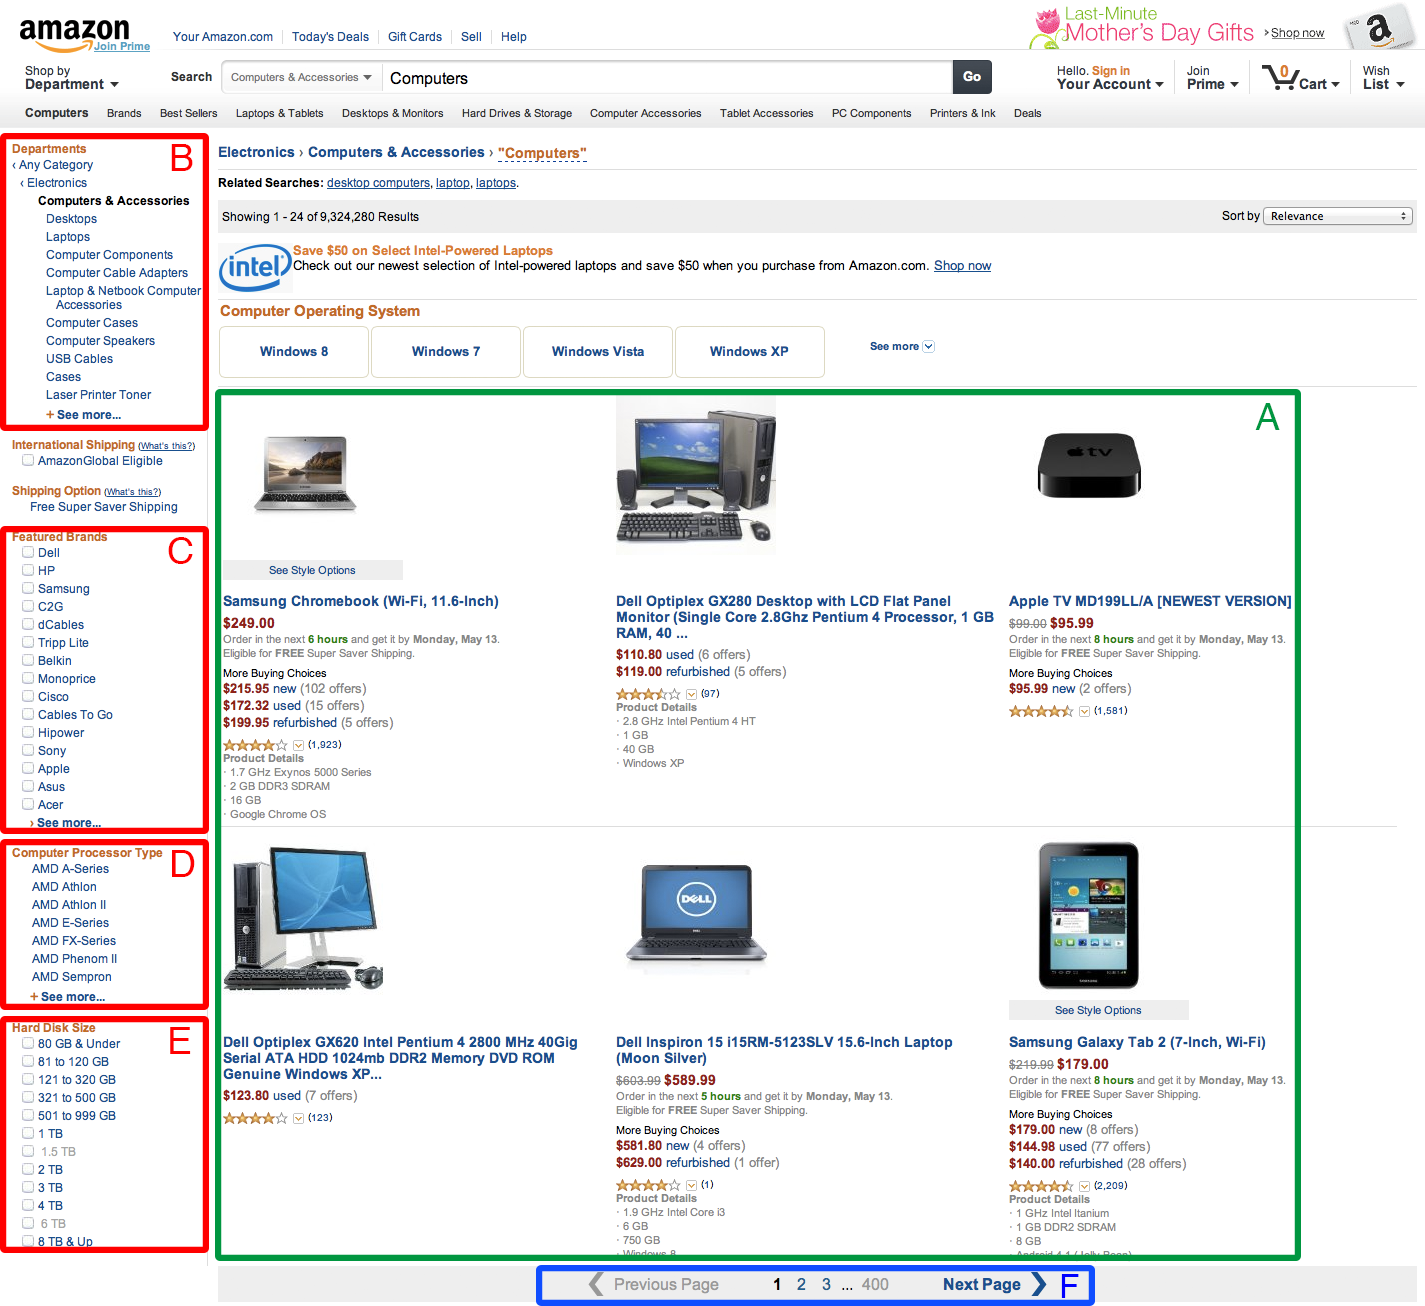
\includegraphics[scale=0.40]{imgs/chap_2/Amazon.png}
\caption{An example of Amazon Web page}
\label{fig:amazon1}
\end{figure}

Figure~\ref{fig:amazon1} shows an Amazon web page returned for the query \textit{Computer}. In such page it is possible identify several groups of structural data. In particular, links in structured data that describe the product listing (i.e., box A) allow us to obtain key information related to real-world entities (e.g., computers) while links contained in the other structured data (boxes B, C, D, E, F) allow us to navigate the organization of the website and identify meaningful connections among objects (e.g., identify computers belongs to the same brand).

Extracting such data records is useful in several application domains because it enables us to obtain and integrate data from multiple sources (websites and web pages) to provide value-added services, e.g., customizable web information gathering, comparative shopping, meta-search, etc. With more and more companies and organizations disseminating information on the Web, the ability to extract such data from
web pages is becoming increasingly important.

%Differently from traditional textual documents, structured data in web pages are enriched by hyperlinks that enable information to be splitted in multiple and interdependent web pages. These hyperlinks can be used to identify collections real-world entities (e.g., web pages of courses, professors, products, news, etc) and relationships among entities.  Figure~\ref{} shows an Amazon web page returned for the query \textit{Computer}. In such page it is possible identify several groups of structural data. In particular, links in structured data that describe the product listing allow us to obtain key information related to real-world entities (e.g., computers) while links contained in the other structured data allow us to navigate the organization of the website and identify meaningful connections among objects (e.g., identify computers belongs to the same brand). 

Although these data are easily identified by humans, machines are not able to directly access to structured data encoded in web pages. Moreover, since web documents are neither well structured such as database nor completely unstructured such as pure textual documents, traditional Data Mining or Text Mining techniques can not be directly applied on structured data encoded in web pages.

%In the first case, Data Mining techniques are based on the assumption that data used to learn models share a common schema and be independent among them. 
In the first case, Data Mining techniques are based on the assumption that data used for learning models share a common schema having well defined tables, attributes (columns), tuples (rows), keys, and constraints. Moreover, such data should be independent among them. 
Web pages break this assumption because structured data do not share a common schema and their hyperlinks define interdependence relationships among web records and web pages. Moreover, web pages are codified in HTML a markup language that, differently from other language markups used to store data such as XML, was projected just for data rendering. Consequently, the Web can be considered a modern legacy system because such a large body of data cannot be easily accessed and manipulated. 

In the second case, Text Mining techniques extract structured data in web pages analyzing recurrent patterns and named entities in word sequences~\cite{Sarawagi:2008}. Existing solutions for plain documents fail to learn accurate models because they are based on assumption that the document collection is written with a consistent writing style (e.g., news articles). Moreover, text mining approaches, considering documents as sequences of words, are not able to extract valuable information from different web page's representations. In fact, differently from textual documents, web pages have multiple representations which provide different information; one is the text representation written in HTML; the other is the visual representation rendered by a web browser. These sources of information are completely ignored by Text Mining approaches. As consequence, they are not able to handle complex information within web elements possessing various semantic roles (e.g., a navigation menu, main content, calendar, table, and logotype) and providing different functionalities (e.g., a link, button, and element with drag-and-drop function)~\cite{Qi:2009}. Finally differently from textual documents, web pages are enriched by hyperlinks that enable information to be splitted in multiple and interdependent web pages. These hyperlinks can be used to identify collections real-world entities (e.g., web pages of courses, professors, products, news, etc) and relationships among entities. Also this information is ignored by Text Mining. 

Consequently, there is a strong need in the computer science field of creating techniques and approaches that, using textual, structural, and visual information of web pages, are able to extract schema from structured data and align the data using that schema. 
Goal of Web Information Extraction is that to transform the Web from a legacy system to the biggest, structured, and easily accessible database. 

%\section{Structured Data in the Web}
%\label{sec:Structured Data in the Web}  
%\color{red}
%A large amount of information from the Web is represent in form of semi-structured data, that is a combination of unstructured text with data having a structure or a schema~\cite{Arasu:2002}. Structured data contained in web pages are typically \textbf{data records} generated dynamically from an underlying structured source like a relational database (e.g., product listing of an Amazon web page) or from a  static template (e.g., menus, navbars, etc.).

%Extracting such data records is useful in several application domains because it enables us to obtain and integrate data from multiple sources (websites and web pages) to provide value-added services, e.g., customizable web information gathering, comparative shopping, meta-search, etc. With more and more companies and organizations disseminating information on the Web, the ability to extract such data from web pages is becoming increasingly important.

%Differently from traditional textual documents, structured data in web pages are enriched by hyperlinks that enable information to be splitted in multiple and interdependent web pages.
%These hyperlinks can be used to identify collections real-world entities (e.g., web pages of courses, professors, products, news, etc) and relationships among entities. 
%Figure~\ref{} shows an Amazon web page returned for the query \textit{Computer}. In such page it is possible identify several groups of structural data. In particular, links in structured data that describe the product listing allow us to obtain key information related to real-world entities (e.g., computers) while links contained in the other structured data allow us to navigate the organization of the website and identify meaningful connections among objects (e.g., identify computers belongs to the same brand). 

%As mentioned above, since web documents are neither well structured such as database nor completely unstructured such as pure textual documents, traditional Data Mining or Text Mining techniques can not be directly applied on structured data encoded in web pages.
%In the first case, Data Mining techniques are based on the assumption that data used to learn models share a common schema and be independent among them. 
%In the first case, Data Mining techniques are based on the assumption that data used for learning models share a common schema having well defined tables, attributes (columns), tuples (rows), keys, and constraints. Moreover, such data should be independent among them. 
%Web pages break this assumption because they contain heterogeneous data and their hyperlinks define interdependence relationships. Moreover, web pages are codified in HTML a markup language that, differently from other language markups used to store data such as XML, was projected just for data rendering. From this reason, the Web can be considered a modern legacy system, since such a large body of data cannot be easily accessed and manipulated. 
%In the second case, Text Mining techniques fail to learn accurate models on web pages because they require collection of documents written with consistent styles (e.g., news articles) and are not able to handle complex information with elements possessing various semantic roles (e.g., a navigation menu, main content, calendar, table, and logotype) and providing different functionalities (e.g., a link, button, and element with drag-and-drop function)~\cite{Qi:2009}. 
%In fact, differently from textual documents, web documents have multiple representations which provide different information. One is the text representation written in HTML; the other is the visual representation rendered by a web browser. Text Mining algorithms focus on the text representation while ignore the visual information.   

%Consequently, there is a strong need in the computer science field of creating techniques and approaches that, using textual, structural, and visual information of web pages, are able to extract schema from structured data and align the data using that schema. 
%Then the goal of Web Information Extraction is that to transform the Web from a legacy system to the biggest, structured, and easily accessible database. 
\section{The role of Information Extraction}
\label{sec:The role of Information Extraction}
%\color{green} introduzione a IE, trovare strutture nascoste nelle pagine web (vedi anche abstract dakkar)
%    e.s. strutture nelle tabelle
%         strutture nelle liste\\
\color{red}
Information Extraction born originally as a natural language processing task used to extract relevant information both from structured text with tabular information and from free text such as news articles~\cite{Eikvil:1999}. Goal of Information Extraction is to identify patterns involving syntactic relationships between words or semantic classes of words. Extracted patterns can be used generate a relation of k-tuple (where k is the number of attributes in a record) or a complex object with hierarchically organized data~\cite{Chang:2006}.
An application example is to extract from a terrorist attack article key information about perpetrators, their affiliation, victims, location, etc \cite{Pio:2014}. 

With the growth of the Web researches tried to apply information extraction techniques on web pages. %As said in the previous section a web page is considered structured if each attribute in a data record can be correctly extract based on some uniform syntactic clue, such as delimiters, visual alignments, etc, while it is considered semi-structured if it is not possible extract directly a complete schema due data records with missing attributes, attributes with multiple values, attribute permutations, and exceptions. 
%Figure~\ref{fig:ebay} shows an example of semi-structured web page with several missing attributes in data records (e.g., item description, original price, etc.).  
%\begin{figure}[t!]
%\centering
%\includegraphics[scale=0.25]%{imgs/chap_1/ebay_semiStructuredSchema.png}
%\caption{An example of semi-structured web page}
%\label{fig:ebay}
%\end{figure}
As said in the previous section, web pages differ from textual documents for several aspects, such as absence grammatical structures, presence of hyperlinks, etc.
For this reason, traditional information extraction tools which use linguistic knowledge to extract key information are not suitable for web pages. For example, most of structured data in web pages are rendered using regular HTML tags patterns and information are splitted in interconnected web pages. For these web pages the analysis of regularity on their visual and structural representation and the analysis of the graph behind the website can be used for extracting structured data more accurately and efficiently than natural language processing methods. 

Information extraction systems on the Web require to solve five distinct problems:
\begin{itemize}
\item \textbf{Navigation problem}: finding target web pages, i.e., pages containing data to extract in a website following hyperlinks. Websites, especially data intensive websites, contain both target pages and navigational pages (i.e., web pages contain hyperlinks to target pages or to other navigational pages). A system for extracting structured data should explore web pages in a way to minimize the search space to target pages and as less navigation pages as possible.  
\item \textbf{Data extraction problem}: extracting relevant data records from web pages. Solutions to extract data records should analyze structural and visual properties of web elements to find recurrent patterns which describe data records.
\item \textbf{Schema synthesis problem}: generating schema behind extracted data- records. In this case  solutions are needed to extract and align attributes from data records. These solutions should be able to handle missing values, values embedded in plain text paragraphs, values hierarchically organized, etc.  
\item  \textbf{Data mapping}: aggregating data from several websites. This requires data be homogenized since different websites can follow different conventions for naming things, for expressing measured units (e.g. currency, weight of a product, etc.), etc.. Mapping discrete values (e.g. company names) into a standard format and transforms measured values in a common unit improves the quality of the extracted data. 
\item \textbf{Data integration}: merging data from separate web pages. Some websites, especially websites with a large amount of data (e.g. Ebay, Amazon, etc.), split structured data on multiple web pages for avoiding to overload a single page with too much information (e.g., splitting the products listing using the pagination list). Other times information about a single data record are splitted on multiple web pages (e.g., reviews of a product and  main information about the product self are stored on two different 
web pages). 
Large scale programs able to fetch tens of thousands of web pages per second are called \textit{crawler, spiders, web robots, or bots}.
\end{itemize}

To extract structured data from the Web, several types of wrappers have been created. A wrapper can be defined as a program that extracts structured data of a particular information source and translates them into a relational form~\cite{Kushmerick:1997}.
Existing wrappers can be categorized in three main groups:
\begin{itemize}
\item \textbf{Manual wrapper}: it involves the writing of ad hoc code. Human programmers identify syntactic patterns to extract structured data analyzing source codes (i.e. HTML code) of web pages and understanding their structure. Although this approach is simple, it suffers several disadvantages due Web features. The first drawback is due by heterogeneity and dimension of the Web; manual wrappers are not scalable %to a large number of websites 
because websites and web pages with different structures require different wrappers. Moreover, the Web is a dynamic environment where web pages are created, destroyed and modified; wrappers can not automatically adapt to these changes since they are based on a specified grammar and manual maintenance has high cost.  
\item \textbf{wrapper induction}: it consists in the automatic wrappers construction based on inductive learning methods. The first wrappers were created around 1995-1996. In this case,  supervised learning approaches are used to automatically generate rules which are then used to extract structured data from unseen web pages. Wrappers based on induction learning can be classified as \textit{zero-order} or \textit{first-order} depending on the inductive learning method used~\cite{Eikvil:1999}. Wrappers constructed using zero-order learning methods learn models in form of couples \textit{attribute-values}, that is, from database point of view as disconnected relations. Differently from zero-order wrappers, first-order wrappers are able to learn models in form of first-order predicates which describe relations and associations between these relations.   

The accuracy of learned rules, and consequently the accuracy of this type of wrappers, strongly depends both the number and the quality of examples (i.e. manually labeled pages and data records). Wrappers generated using supervised learning require a high cost for manual labeling of examples, for generating wrappers from websites with different structure, and for the maintenance in case changes in the websites structure.
\item \textbf{automatic extraction}: it consists in the automatic wrappers construction based on unsupervised learning. Differently from the previous approaches it is not required the manual labeling effort. This makes wrappers scalable to a large amount of websites and easily maintainable. Modern wrappers are based on this approach.
\end{itemize} 

\section{The role of information network analysis}
\color{green}
% Web as Heterogeneus Information Network
%\color{green}
%https://books.google.it/books?id=yqOeBQAAQBAJ&pg=PA7&lpg=PA7&dq=browse+search+navigate+paradigms+web&source=bl&ots=avDgal_C_I&sig=ZvEpsTbNffjgs0ug18M2KbvegaA&hl=it&sa=X&ved=0ahUKEwiy8uLw9rXJAhVIDSwKHWw_Dv8Q6AEIOTAD#v=onepage&q=browse%20search%20navigate%20paradigms%20web&f=false
\color{red}
    %Information networks are ubiquitous and form a critical component of modern information infrastructure. Most of data or informational objects, individual agents, groups, or components are interconnected or interact with each other, forming numerous, large, interconnected, and sophisticated networks.
%The Web can be considered the largest, complex, and unexplored information network. In fact, it contains billion of shared and public availabe documents related to a complete range of topics, from product to financial, public-record, scientific, hobby-related, and government.\\

Nowadays, most real phenomena can be represented as information networks, that is graphs where the nodes are real-world entities interconnected and interacting among them. 
Formally an information network can be defined as follow \cite{Sun:2012}:
\begin{definition}
\label{def:network}\textbf{Information Network:}
is defined as a directed graph $G = ( V , E )$ with an object type mapping function $\tau : V \rightarrow A$ and a link type mapping function $\phi : E \rightarrow R$, where each object $v \in V$ belongs to one particular object type $\tau (v) \in A$ , each link $e \in E$
belongs to a particular relation $\phi(e) \in R$ , and if two links belong to the same relation type, the two
links share the same starting object type as well as the ending object type. 
\end{definition}

\begin{figure}[h]
\centering
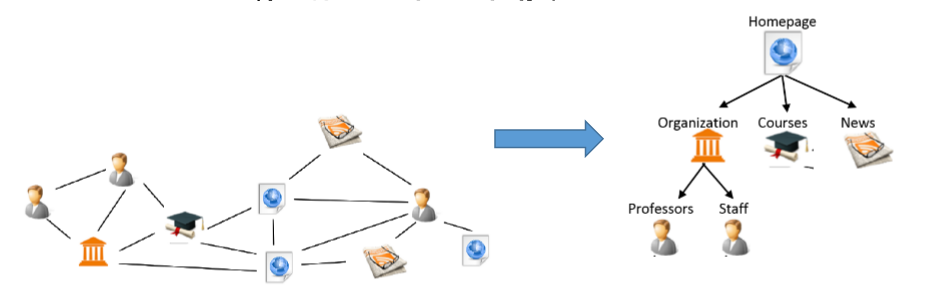
\includegraphics[scale=0.40]{imgs/chap_1/informationNetwork1.png}
\caption{An example of an information network of a website where nodes are web pages related to different entity types (e.g. people, news, organizations) and edges are hyperlinks}
\label{fig:informationNetw}
\end{figure}


The analysis of information networks %, or their special kinds, such as social networks \cite{Wasserman:1994} and the Web, 
has gained extremely wide attentions nowadays from researchers in several fields such as
computer science, social science, physics, economics, bioinformatics, and so on, with exciting discoveries and successful applications across all the disciplines. Goal of information network analysis is to extract patterns or regularities in relationships among interacting units which represent the structure of the network. 
For example, the application Data Mining or Graph Mining techniques on information networks allows researches to discover latent structures among nodes, such as the topics and communities they are involved in, the roles that different types of nodes play in these topics and communities, and the relations they potentially have with each other. These approaches can be used in the context of the Web for combining intra-page information (e.g. textual content, HTML structure) with inter-page information which describe the topological structure of websites.

Although several methods and approaches exist for extracting knowledge from the information networks, most of the existing studies are based on the assumption that  networks are homogeneous. %, that is nodes and relationships are of the same type. 
However, real information networks contain heterogeneous and structured data (e.g., relational database data) \cite{Sun:2012}. Although a single link in the network could be noisy, unreliable and sometimes misleading, valuable knowledge about the structure of networks can be discovered reliably analyzing massive connections between objects~\cite{Kargupta:2008}.
\section{Outline of the thesis}
%Vedere pagina 16 http://www0.cs.ucl.ac.uk/staff/J.Zhu/thesis.pdf

In this thesis I investigate the principles and methodologies for discovering novel and valuable knowledge from the Web.  I propose models and algorithms which exploit the main features of web pages and websites for extract structured information encoded in one or more web pages or hidden in the link structure of websites. Proposed methods involve several fields, ranging from Web Information Extraction to Information Network Analysis, Sequential Pattern Mining, Web Structure and Content Mining. Moreover, the methods and approaches analyzed and implemented in this thesis can contribute to give a structure to the Web exploiting and discovering properties and interactions among web pages that were previously unknow

%contibute to evaluate interactions among web pages, organize the content of websites and understand their structure. 

%and can contribute to give a structure to the Web and explore properties and interactions among web pages that were previously unknow. 

The major contributions are threefold. First, I propose a novel solution to extract structured data in form of \emph{web lists} splitted on multiple web pages. Although this task has been studied extensively, existing approaches are based on the assumption that lists are wholly contained in a web page. They do not consider that many websites span structured data of same semantic class (e.g. books, professors, product listing)  on several web pages and show for each of these only a partial view. Proposed method combine information intra-page (i.e web lists) and extra-page information (website structure) to extract a complete collection of structured data belonging to the same semantic class.

Second, a method to automatically discover sitemaps is realized. Actually  sitmaps are manually generated by web designer or automatically extracted by infomation network analysis tools. In the former, manual approaches extract static and deeper (with respect to automatic methods) hierarchies which are not able to capture evolutions in the website (e.g. generation of new sections, deletion of existing web pages, etc.). This makes sitemaps helpless and confusing for users after few time. In the latter, existing solution extract only a flat list of website's urls that do not show the hierarchical structure of a website or use only web pages' content ingnoring the website's link structure. Differently from existing automatic solutions, the proposed approach  is both automatic and effective. It explores navigation systems (e.g. menu, nav-bar, content list, etc.) contained in a website and exploits recurrent patterns of navigation systems to discover rich hierarchies that unveil relationships among web pages (e.g. relationships of super/sub category). For this scope, a novel sequential \emph{closed} pattern mining algorithm, called CloFAST, is implemented. CloFAST combines a new data representation of a sequence dataset  with a novel one-step technique to both generate sequences and to prune the search space. These features allows CloFAST to drastically reduce the number of
intermediate subsequences and then reduce the computational complexity of the sequence generation process while preserving the same
expressive power of patterns extracted by means of existing algorithms. Reducing the computational complexity of algorithms used the Web context is foundamental task.

Third, I focus on another challenging task in Web Mining: clustering of web pages. Web pages are characterized by different roles and several representations, based on textual, hyperlink and HTML formatting (i.e. HTML tags and visual) properties. Existing clustering algorithms use these information almost independently, mainly because it is difficult to combine them. Proposed solution is intended to be a contribution on clustering of web pages in a website by combining all this features into a single vector space representation. 






  

 


